\section*{Animal Faces}
\begin{frame}{About Dataset}
    \begin{table}
        \centering
        \begin{tabular}{|c|c|}
            \hline
            \textbf{Dataset} & \textbf{Animal Faces} \\
            \hline
            \textbf{Size} & 512x512 \\
            \hline
            \textbf{Training Images} & 14630 \\
            \hline
            \textbf{Validation Images} & 1500 \\
            \hline
            \textbf{Number of Classes} & 3 \\
            \hline
        \end{tabular}   
    \end{table}
    For all out experiments we have resized our images to 128x128.
\end{frame}

\begin{frame}{Training for cats only}
    We trained VAE for 5153 cat images and used 500 images for validation. We trained over 40 epochs. Here are the results:
    \begin{figure}
        \centering
        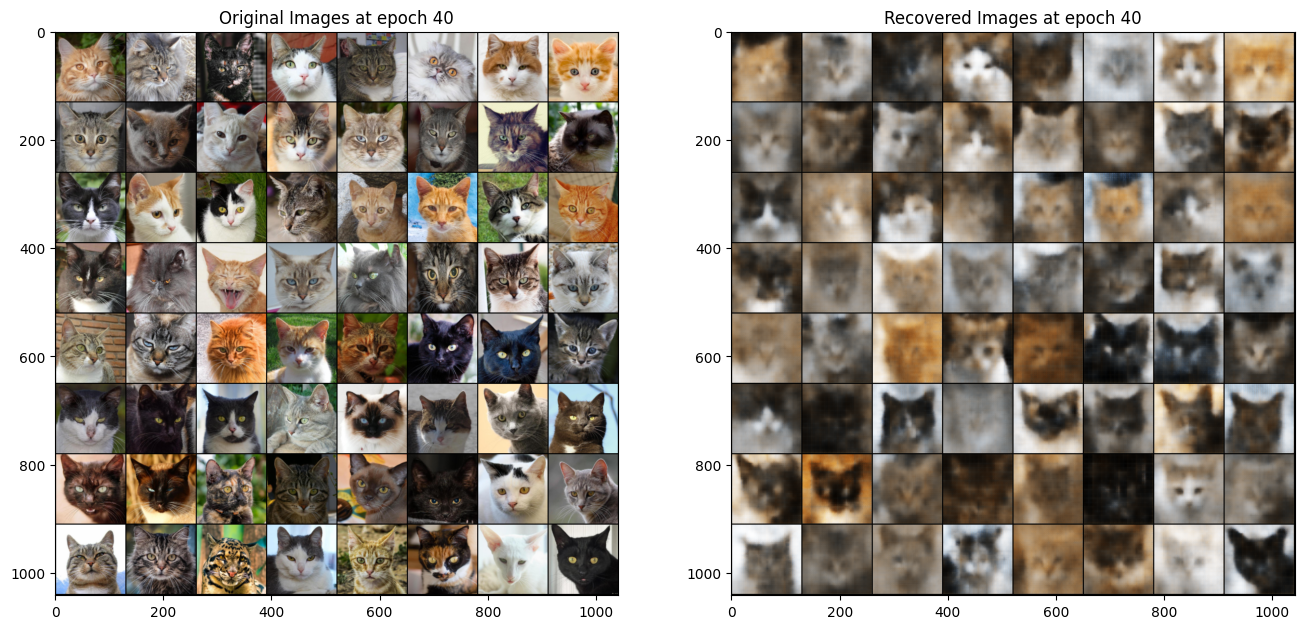
\includegraphics[width=0.8\textwidth]{../ReportNeurips/catsReconstruct.png}
        \caption{Reconstructions of VAE on Cat dataset}
    \end{figure}
\end{frame}

\begin{frame}{Generation}
    \begin{figure}
        \centering
        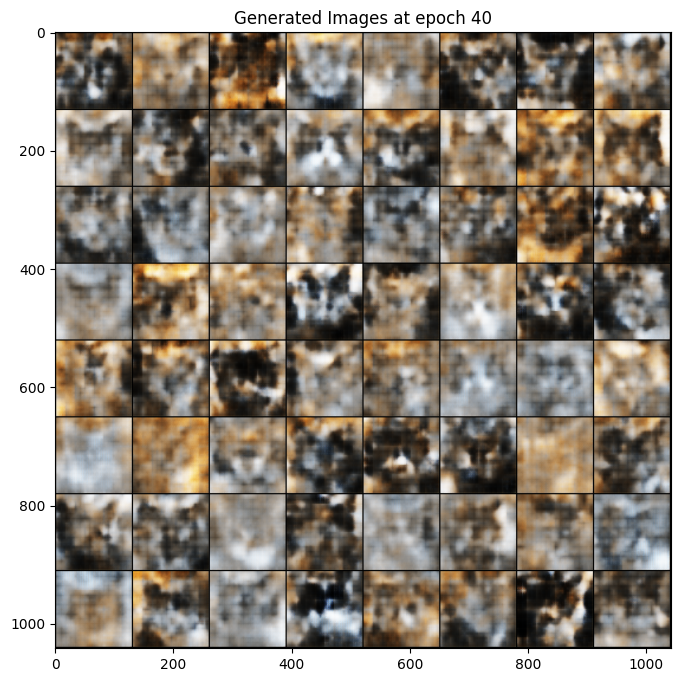
\includegraphics[width=0.55\textwidth]{../ReportNeurips/CatGeneration1.png}
        \caption{Generation of new cat images using VAE}
    \end{figure}
\end{frame}

\begin{frame}{Loss Curves}
    \begin{figure}
        \centering
        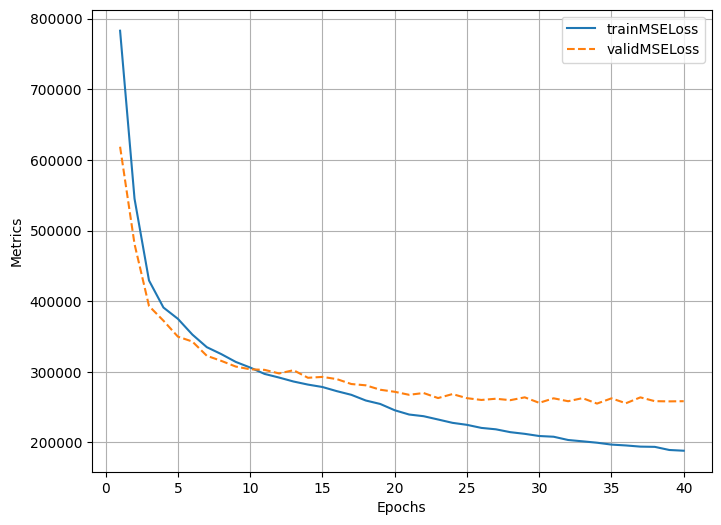
\includegraphics[width=0.6\textwidth]{../ReportNeurips/catLoss.png}
        \caption{Loss Curves for VAE on Cat dataset}
    \end{figure}
\end{frame}

\begin{frame}{Training for wild animals only}
    We trained VAE for 4738 images of wild animals and used 500 images for validation. We trained over 70 epochs.
    \begin{figure}
        \centering
        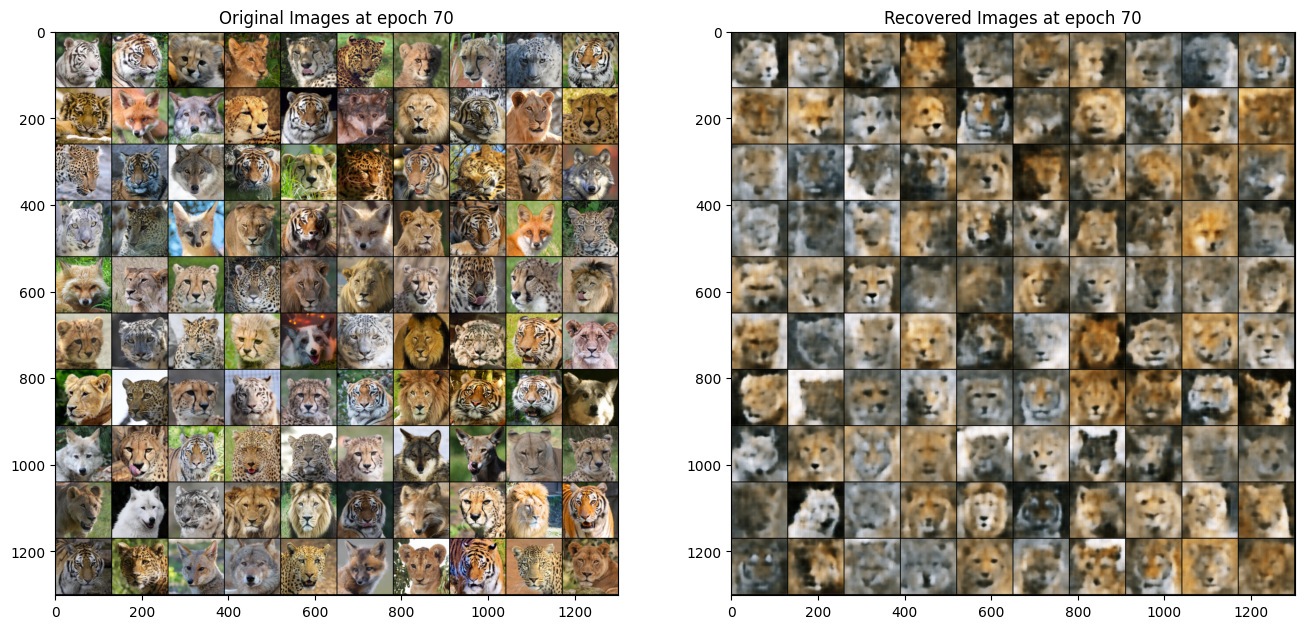
\includegraphics[width=1\textwidth]{../ReportNeurips/wildanimal.png}
        \caption{Reconstructions of VAE on Wild Animals}
    \end{figure}
\end{frame}

\begin{frame}{Generation}
    \begin{figure}
        \centering
        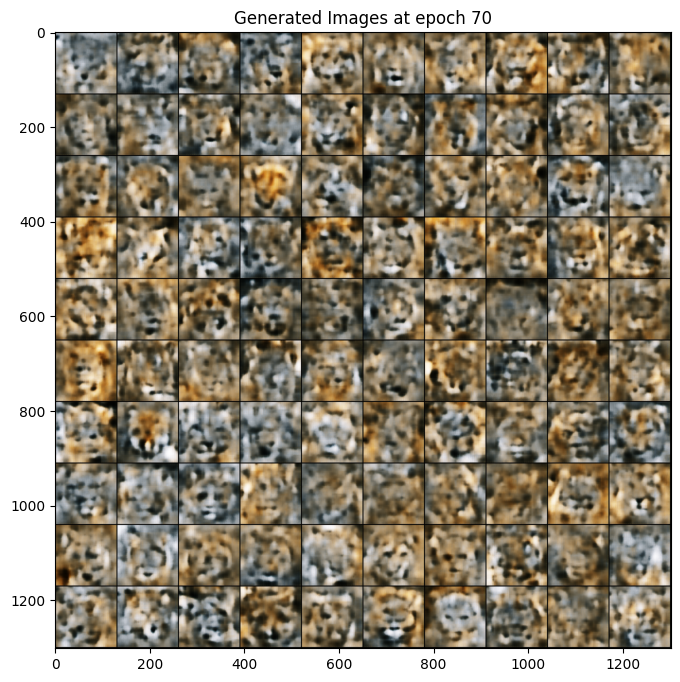
\includegraphics[width=0.55\textwidth]{../ReportNeurips/wildanimal1.png}
        \caption{Generation of new wild animal images using VAE}
    \end{figure}
\end{frame}

\begin{frame}{Loss Curves}
    \begin{figure}
        \centering
        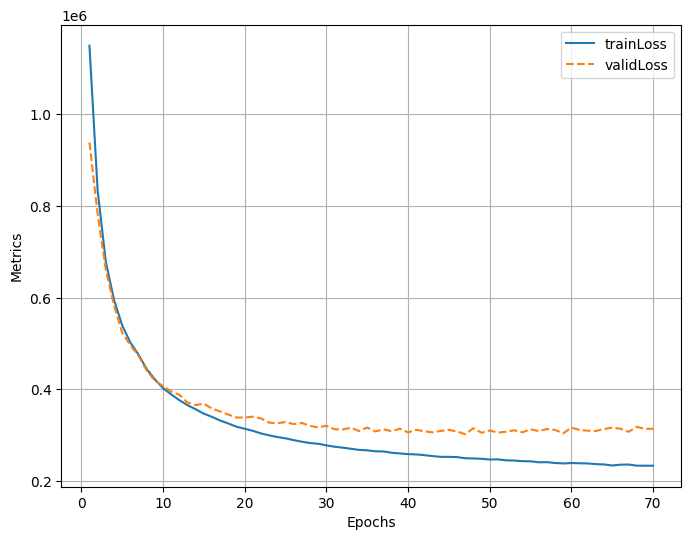
\includegraphics[width=0.6\textwidth]{../ReportNeurips/losscurve2.png}
        \caption{Loss Curves for VAE on Wild Animals}
    \end{figure}
\end{frame}

\begin{frame}{Training on full dataset}
    We trained VAE for 14630 images of animals and used 1500 images for validation. We trained over 100 epochs.
    \begin{figure}
        \centering
        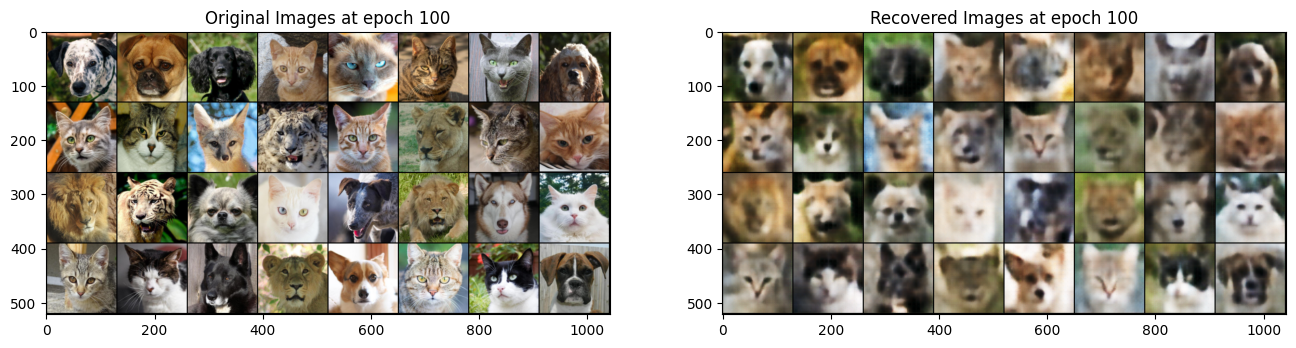
\includegraphics[width=1\textwidth]{../ReportNeurips/reconstructfull.png}
        \caption{Reconstruction of VAE on Animal Face Dataset}
    \end{figure}
\end{frame}

\begin{frame}{Generation}
    \begin{figure}
        \centering
        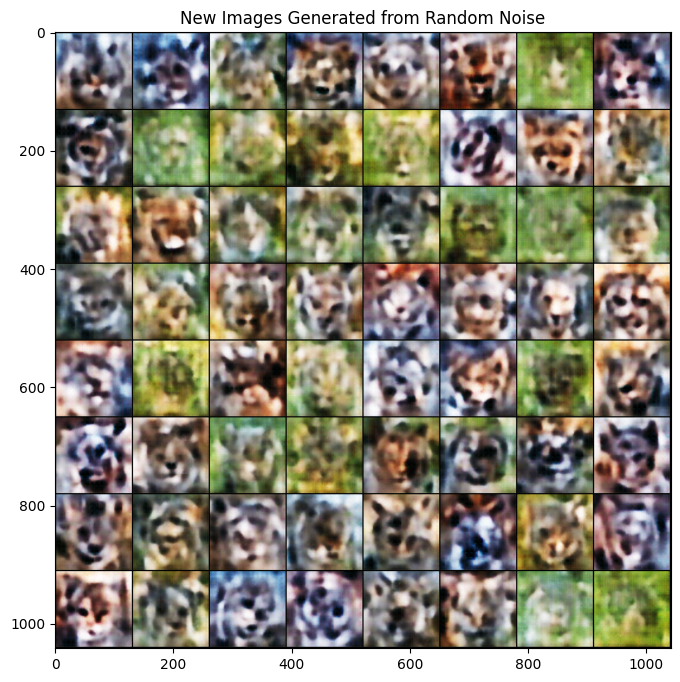
\includegraphics[width=0.55\textwidth]{../ReportNeurips/generationFull.png}
        \caption{Generation of new animal face images using VAE}
    \end{figure}
\end{frame}

\begin{frame}{Loss Curve 1}
    Here are plot for Train Loss and Validation Loss for VAE on Animal Face Dataset.
    \begin{figure}
        \centering
        \includegraphics[width=0.6\textwidth]{../ReportNeurips/losscurve.png}
        \caption{Loss Curves for VAE on Animal Face Dataset}
    \end{figure}
\end{frame}

\begin{frame}{Loss Curve 2}
    Here are plot for KL Divergence Loss during training and validation for VAE on Animal Face Dataset.
    \begin{figure}
        \centering
        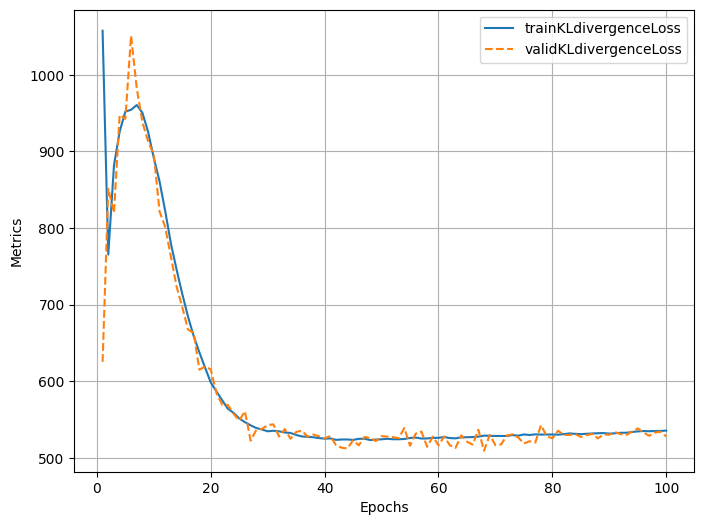
\includegraphics[width=0.6\textwidth]{../ReportNeurips/klLoss.png}
        \caption{KL Divergence Loss for VAE on Animal Face Dataset}
    \end{figure}
\end{frame}

\begin{frame}{Frechet Inception Distance}
    We took randomly choosen 2000 images resized to 128x128 from training set and generated 2000 images using VAE. Our calculated FID score is 269.98.
    \begin{figure}
        \centering
        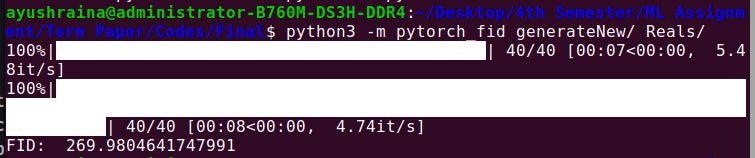
\includegraphics[width=0.6\textwidth]{../ReportNeurips/FID.png}
        \caption{Frechet Inception Distance for VAE on Animal Face Dataset}
    \end{figure}
\end{frame}

\begin{frame}{Key Takeaways}
    \begin{itemize}
        \item Importance of Learning Rate.
        \pause
        \item Importance of Batchsize when training with GPU's.
        \pause
        \item More is KL weight, more better the generation, but reconstruction may suffer.
        \pause
        \item Number of epochs is also important to prevent overfitting sometimes.
        \pause
        \item Playing with architecture can also give better results.
    \end{itemize}
\end{frame}

\begin{frame}{Some more results}
    These are the results that we obtained during experiments but we lost the parameters onwhich these were generated.
    \begin{figure}
        \centering
        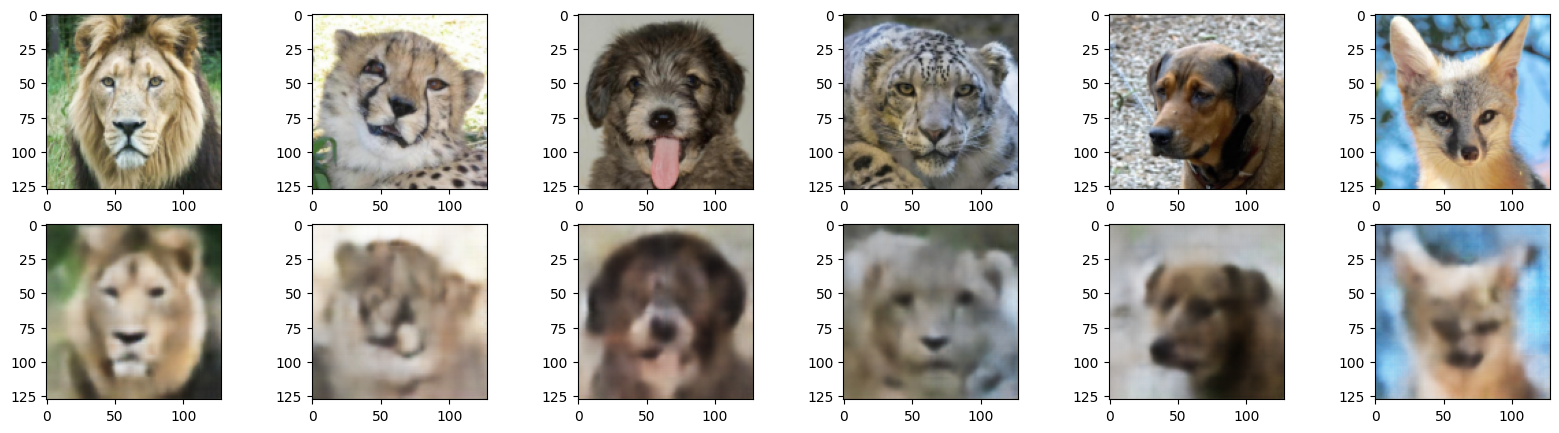
\includegraphics[width=0.8\textwidth]{../lion.png}
        \caption{Reconstruction}
    \end{figure}
\end{frame}

\begin{frame}{Some more results}
    \begin{figure}
        \centering
        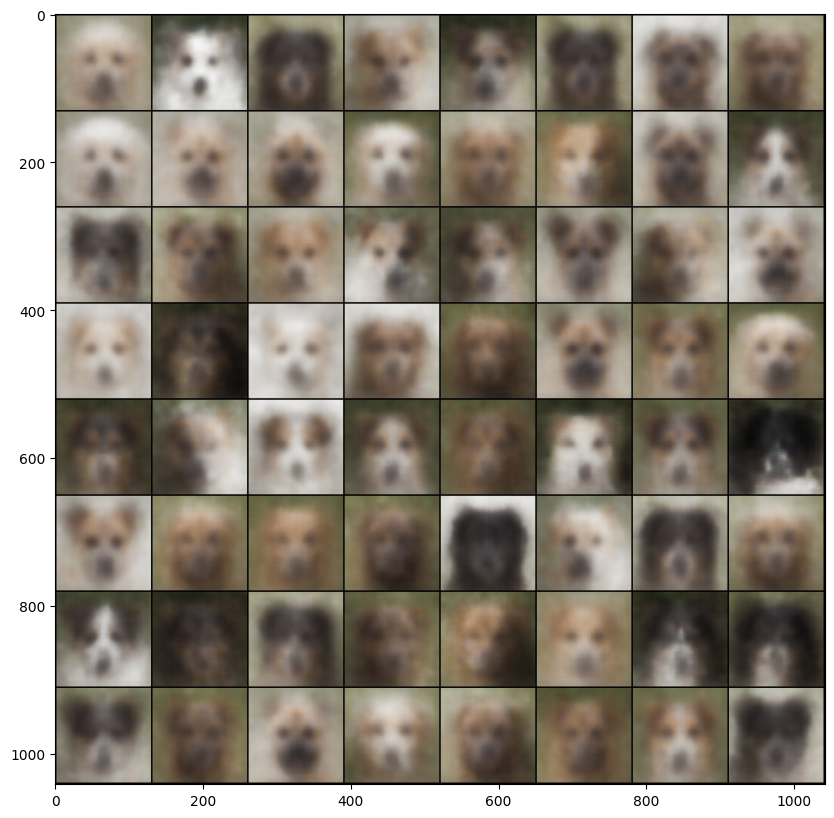
\includegraphics[width=0.6\textwidth]{../dogs1.png}
        \caption{Generation}
    \end{figure}
\end{frame}
